% \usepackage[T1]{fontenc}

% \usepackage[utf8]{inputenc}

\section{Анализ предметной области и постановка задачи}

При проектировании программного продукта, который решает реальные задачи пользователя, очень важно выяснить главный функционал и свойства продукта, чтобы сервис отвечал запросам пользователей и производство продукта было оправдано.

Требования к ПО определяют, какие свойства и характеристики оно должно иметь для удовлетворения потребностей пользователей и других заинтересованных лиц. Однако сформулировать требования к сложной системе не так легко.
В большинстве случаев будущие пользователи могут перечислить набор свойств, который они хотели бы видеть, но никто не даст гарантий, что это — исчерпывающий список.
Кроме того, часто сама формулировка этих свойств будет непонятна большинству программистов.

Чтобы ПО было действительно полезным, важно, чтобы оно удовлетворяло реальные потребности людей и организаций, которые часто отличаются от непосредственно выражаемых пользователями желаний.
Для выявления этих потребностей, а также для выяснения смысла высказанных требований приходится проводить достаточно большую дополнительную работу, которая называется анализом предметной области или бизнес-моделированием, если речь идет о потребностях коммерческой организации.
В результате этой деятельности разработчики должны научиться понимать язык, на котором говорят пользователи и заказчики, выявить цели их деятельности, определить набор задач, решаемых ими.
В дополнение стоит выяснить, какие вообще задачи нужно уметь решать для достижения этих целей, выяснить свойства результатов, которые хотелось бы получить, а также определить набор сущностей, с которыми приходится иметь дело при решении этих задач.
Кроме того, анализ предметной области позволяет выявить места возможных улучшений и оценить последствия принимаемых решений о реализации тех или иных функций[2].

После этого можно определять область ответственности будущей программной системы — какие именно из выявленных задач будут ею решаться, при решении каких задач она может оказать существенную помощь и чем именно.
Определив эти задачи в рамках общей системы задач и деятельностей пользователей, можно уже более точно сформулировать требования к ПО.

Далее приводится анализ сведений, которые влияют на формулирование требований, выбор архитектуры и дальнейшее проектирование и разработку программного средства.

\subsection{Постановка задачи}

Задача данного дипломного проекта, является проектирование  и реализация программного обеспечения для автоматизации процесса сдачи вещей в аренду.

Помимо организации самого процесса покупки и продажи товара в аренду, в приложении должны присутствовать такие функции, как:
\begin{itemize}
  \item Возможность регистрации пользователя в системе;
  \item Размещение товара на продажу;
  \item Сохранение истории  товарооборота;
  \end{itemize}


\subsection{Электронная коммерция}
В общем случае «система электронной коммерции» представляет собой определенную Интернет-технологию, предоставляющую участникам системы следующие возможности[3]:
\begin{itemize}
  \item Производителям и поставщикам товаров и услуг различных категорий - представить в сети Интернет товары и услуги (в том числе онлайновые услуги и доступ к информационным ресурсам), принимать через Интернет и обрабатывать заказы клиентов;
  \item Покупателям (клиентам) - просматривать с помощью стандартных Интернет-браузеров каталоги и прайс-листы предлагаемых товаров и услуг и оформлять через Интернет заказы (заявки, запросы) на интересующие товары и услуги.
  \item
\end{itemize}

Важной (но необязательной) составляющей систем электронной коммерции являются системы проведения электронных платежей - в этом случае одним из участников системы становится банк.

В числе функциональных возможностей, реализуемых системами электронной коммерции, можно выделить следующие:
\begin{itemize}
  \item Оформление заказов по каталогам и прайс-листам (заказы хранятся в единой базе данных);
  \item Связь Интернет-приложений с внутренней системой делопроизводства;
  \item Саморегистрация пользователей;
  \item Поддержка как локального, так и удаленного (через Интернет) администрирования;
  \item Возможность продаж через Интернет товаров различных категорий;
  \item Обработка заказов по стандартной схеме (регистрация, поставка, отчетно-финансовые документы);
  \item Проведение онлайновых платежей.
\end{itemize}

Электронную коммерцию можно подразделить на 3 категории:
\begin{itemize}
  \item Бизнес-бизнес (business-to-business);
  \item Бизнес-потребитель (business-to-consumer);
  \item Бизнес-администрация (business-to-administration).
\end{itemize}

Примером из категории бизнес-бизнес может служить компания, использующая сеть для заказов поставщикам, получения счетов и оплаты.
Эта категория электронной коммерции успешно складывалась в течении нескольких лет, с частичным использованием технологии электронного обмена данными - EDI (Electronic Data Interchange) в частных сетях или сетях с дополнительными услугами - VAN (Value Added Networks).

Категория бизнес-потребитель - это электронная розничной торговля. Эта категория сильно расширила свои рамки с появлением WWW.
На сегодняшний день в Internet открыто множество магазинов, предлагающих потребителям всевозможные товары, от печенья и вина до компьютеров и автомобилей.

В категорию бизнес-администрация входят все сделки, заключаемые между компаниями и правительственными организациямих[4].
Например, в США информация о планируемых правительством закупках публикуется в Internet и компании могут посылать свои предложения электронным способом.
Сегодня эта категория пока находится в зачаточном состоянии, но может быстро разрастись при условии, что правительства используют собственные возможности для поддержки и развития электронной коммерции.
В добавление к объявлениям о закупках, административные органы могут также предлагать возможность электронного обмена при таких операциях, как например, возврат налога на добавленную стоимость.

Электронная коммерция - это составная часть электронного бизнеса, которая обеспечивает выполнение функций маркетинга, оформление заказов товаров и услуг, проведение платежей, выбор и реализацию схемы доставки товара, осуществление послепродажного обслуживания через Интернет.

Преимущества электронной коммерции по сравнению с традиционными видами коммерческой деятельности:
\begin{itemize}
  \item Расширение рынков сбыта для поставщиков и новые возможности выбора для покупателей;
  \item Возможность для поставщика индивидуальной работы с покупателями, а для покупателей – персонально подобранные товары и услуги;
  \item Сокращение или устранение посреднической цепи, соответственно быстрый отклик;
  \item Сокращение издержек – интернет-магазины, имея склады, не требуют торговых залов, многочисленного обслуживающего персонала, снижаются затраты на рекламу, в конечном итоге - снижение цен для покупателей;
  \item Возможность непрерывного контроля за выполнением заказа;
  \item Новые возможности для бизнеса;
\end{itemize}

\subsection{Анализ рынка электронной коммерции}
Объем мирового рынка eCommerce в 2019 году мог достигнуть \$3,46 трлн[5], следует из результатов исследования Internet Retailer.
Согласно анализу экспертов, объем розничных онлайн-продаж в 2016–2019 годах рос в среднем на 20\% в год, в то же время розничные продажи увеличивались всего лишь на 3,5\% в год.

Соответственно, рынок растет, в основном, за счет онлайн-коммерции, делают выводы эксперты. При этом доля интернет-продаж в сфере розничной торговли вырастет с 10,5\% в 2016 году до 16,4\% в 2019 году.

Если подобная тенденция сохранится, то объемы мирового рынка eCommerce превысят объёмы традиционной розницы уже к 2036 году.

По мере того как потребители приобретают уверенность в том, что их ждёт хороший опыт онлайн-покупок, они ищут в интернете товары более высокого качества по более низким ценам.
Также они любят интернет-магазины за широкий выбор товаров.

Уже больше 50\% онлайн-покупателей на Ближнем Востоке, в Африке, Европе и Латинской Америке выбирают товары на иностранных сайтах, следует из опроса PayPal.

67\% ритейлеров считают, что именно трансграничная электронная коммерция является важнейшим источником будущего роста для их компании.
52\% согласны с утверждением, что международная электронная коммерция «подходит им, потому что даёт много международных клиентов".


\subsection{Анализ функций сайта}
Цель сайта необходимо обдумать заранее, с участием всех заинтересованных лиц.
Нужно подробно изучить техническое задание и обговорить все нюансы реализации сайта.

Обычно используются следующие цели:
\begin{itemize}
  \item Просветительский;
  \item Рекламный;
  \item Сервисный;
  \item Коммерческий.
\end{itemize}

Цели определяют навигацию, структуру, дизайн, контент, инструментарий для разработки сайта.
Например, для просветительского и рекламного хорошо подходит Joomla («Джумла»), позволяющий создавать «мощный» контент, сайта интернет-магазина.

Определение функций сайта - сложная и трудоемкая работа.
Функции сайта определяют заказчики, аналитики, веб-дизайнер и веб-программист.

Есть три основные функции любого сайта: маркетинговая, информационная и имиджевая[7].

Информационная функция - предоставление новой информации по необходимой теме, области, проблеме.
Данная функция соблюдает высокие требования: скорость загрузки, полнота и ясность контента, обновляемость и функциональность и др.

Имиджевая функция - формирование образа физического или юридического лица, общественного или политического органа в Интернет.
В данной функции большое внимание уделяется дизайну сайта: содержит логотип, фирменный знак, контактные данные и схему проезда (графическую) и другую необходимую информацию для пользователей.

Маркетинговая функция - продажи или увеличение спроса на товар или услугу.
Требования - ненавязчивость, настройками под ключевые запросы посетителей, анкетирование, анализ статистики, скидки и бонусы и др.

Функции сайта определяет только заказчик. Помочь в этом могут и разработчики.

Анализируя функции сайта можно выделить следующие задачи, который должен выполнять Интернет-сайт:
\begin{enumerate}[label=\arabic*)]
  \item Интернет-ресурс является беспрецедентной возможностью предоставить каждому желающему наиболее полную, адресную, продуманную и оперативную информацию о себе и своих услугах;
  \item Интернет-сайт привлекает в первую очередь целевую аудиторию. Под целевой аудиторией подразумевается та группа пользователей сети Internet, для которой данный сайт будет интересен;
  \item Корпоративный Интернет-ресурс может существенно сократить расходы на традиционную рекламу, если используется параллельно с офлайновыми рекламными инструментами: прессой, наружной рекламой и т.п.;
  \item Для расширения рынка сбыта;
  \item Возможность использовать сайт как корпоративное хранилище информации, данных, с которыми сотрудники могут работать дома, в командировках, которые будут доступны партнерам из других регионов;
  \item Сайт является средством конкурентной борьбы.
  К услугам web-представительств обращается все больше и больше фирм.
  Сайт станет дополнительным преимуществом фирмы перед конкурентами, дополнительным и весьма эффективным орудием конкурентной борьбы.
\end{enumerate}

Качественный сайт - должен не только отвечать всем современным техническим требованиям и пожеланиям целевой аудитории, но и учитывать внутренние и внешние факторы ранжирования (критерии качества сайта с точки зрения поисковых систем).

Ниже будут рассмотрены основные критерии оценки качества современного сайта.

Для того, чтобы создать качественный, современный и эффективный сайт необходимо:
\begin{enumerate}[label=\arabic*)]
    \item Разработать эффективный и привлекательный дизайн, соответствующий всем ожиданиям целевой аудитории и выдержанный в фирменном стиле компании. Если сайт выглядит хорошо, то посетители считают, что и компания должна хорошо работать;
    \item Тщательно продумать "юзабилити" (структура, удобство пользования сайтом).
    Нужно, чтобы каждая страница сайта максимально соответствовала пожеланиям посетителя сайта, чтобы все элементы страницы были расположены в самых удобных местах, чтобы информация на сайте читалась легко, а навигация по сайту и поиск - были интуитивно понятными и простыми.
    Посетитель за минимальное количество времени должен получать то, что он хотел получить от сайта.
    В идеале, он должен сразу делать заказ на сайте или другое необходимое целевое действие;

    \item Использовать современные методы разработки сайта.
    В настоящее время разработку сайта необходимо вести в среде HTML5, с использованием CSS3;
    \item Настроить автоматическую трансформацию (адаптивность) сайта под любые мобильные устройства (телефоны, смартфоны, планшеты и пр.). Эта процедура, с недавнего времени, из разряда желательных - переходит в разряд обязательных;


    \item Создавать качественные "посадочные" страницы для каждого поискового запроса.
    О том, что направлять всех посетителей на главную страницу сайта, неразумно и неэффективно - знают уже многие, но мало кто задумывается над тем, что в идеале - для каждого контекстного объявления, для каждой продвигаемой в поисковой выдаче фразы - на сайте должна существовать так называемая "посадочная" страница, или страница "приземления".
    Эта страница должна максимально быстро и всеобъемлюще отвечать на запрос пользователя, по которому он перешел на сайт.
    После посещения этой страницы у посетителя больше не должно возникать соблазна вернуться к поисковой выдаче и посмотреть другие подобные сайты (сайты конкурентов).
    Именно поэтому нужно четко представлять, что именно хочет увидеть посетитель по каждому ключевому запросу и создать под этот запрос отдельную "специальную" страницу;

    \item Обеспечить интеграцию с соцсетями и возможность оставления отзывов. На сайте должна быть реализована возможность проставлять "лайки" и оставлять отзывы о компании, и её продукции.
    Отзывы, оставленные на страницах сайта, позволяют повысить уникальность однотипных страниц, которые поисковые системы часто принимают за неточные копии друг друга и просто исключают их из индексной базы.
    Наличие ссылок на соцсети, лайков и отзывов - позволяет поисковой системе принять решение о социальной активности компании, и в награду за это - "поднять" сайт компании в поисковой выдаче;
    \item Обеспечить высокую скорость загрузки страниц сайта, защиту от спама, взлома и вирусов.
    Современные поисковые системы большое внимание уделяют техническому состоянию сайта.
     Если сайт заражен вирусом, скорость загрузки его страниц невелика, или используются устаревшие технологии создания сайта - высоких позиций в выдаче поисковой системы ожидать не стоит;
    \item После запуска сайта проводить глубокую аналитическую работу, и непрерывно дорабатывать сайт с учетом выявленных технических, структурных, функциональных и иных недочетов, а также поведенческих особенностей использования сайта.
  \end{enumerate}

С точки зрения рассмотрения сайта, как сервиса для предоставления услуг в сфере электронной коммерции, сайт должен иметь такие функции как:
\begin{enumerate}[label=\arabic*)]
    \item Поисковые функции и опции
    \begin{enumerate}[label=\arabic*)]
        \item Поиск товаров – подразумевает наличие функций для поиска товара в каталоге товаров интернет магазина.
        Обычно это поисковая строка на всех страницах интернет магазина.
        В большинстве случаев поиск по сайту выводит информацию по точному вхождению, то есть полному совпадению поискового запроса с найденной информацией.
        Например, если посетитель задаёт запрос «телевизор №N» то он найдёт данный товар, если на сайте есть страница товара с текстом (названием), который точно содержит «телевизор №N»;
        \item Сортировка товаров– подразумевает функцию упорядочивания товаров в каталоге по различным параметрам: цена (от дешевых товаров к дорогим, и наоборот), наименование (по алфавиту наименований), рейтинг (при наличии функции рейтинговой оценки);
        \item Фильтрование и подбор товаров – подразумевает выбор из каталога товаров по нужными параметрам: цвет, размеры, вес и т.д.;
        \item Сравнение товаров. Создание в магазине листа сравнений позволит отобрать нужные товары и определиться с конечным выбором;
    \end{enumerate}
    \item Доставка — нельзя утверждать, что функционал интеграции со сторонними службами доставки крайне необходим для интернет-магазина, т.к. во многих интернет-магазинах товары привозит штатный курьер, а то и сам владелец магазина.
    Однако, использование этого модуля, а главное предоставление возможности выбора способа доставки, повышает лояльность со стороны пользователя и позволяет расширить географию дистрибуции товара;
    \item Оплата — аналогично предыдущему пункту этот функционал не претендует на первые места, однако очень приветствуется пользователями.
    Не всем клиентам удобно оплачивать заказ курьеру или при самовывозе, поэтому подключение системы оплаты на сайте будет отличным шагом для развития интернет-магазина.
    Единственное, что к вопросу подключения данного инструмента мы рекомендуем подходить осторожно;
    \item Личный кабинет клиента — закрытая часть сайта, где хранится история заказов пользователя, а также информация о его адресах доставки и других персональных данных.
    Интернет-магазин может обходиться и без личного кабинета, но наличие данного функционала позволяет упростить клиенту осуществление повторных заказов в магазине, а также дает возможность вовлекать его в различные программы лояльности.
\end{enumerate}


\subsection{Обзор существующих аналогов}
На территории РБ имеется большое количество сервисов для аренды вещей, однако все они относятся к единственным категориям товаров, например: приставки, холодильники, одежда, машины.
Но был найден сервис, который может выступать аналогом в разрабатываемому приложению - R24.by, стартовая страница которого представлениа на рисунке \ref{analogue:start} - он и будет рассмотрен ниже.

R24 - информационный каталог[8], в котором сотни арендодателей предлагают напрокат свои самые разнообразные товары: от небольших украшений и игрушек до крупногабаритной строительной техники и морских контейнеров.
Сайт создан для того, чтобы упростить людям поиск прокатных товаров.
Здесь можно сравнить цены и предложения от множества компаний и сделать правильный выбор.

Наиболее востребованные товары, которые арендуют на R24:
\begin{itemize}
  \item Легковые авто напрокат;
  \item Аренда спецтехники;
  \item Прокат велосипедов;
  \item Аренда строительного оборудования.
\end{itemize}

\begin{figure}[!htb]
  \centering
      \subfloat[Верхняя часть стартовой страницы r24.by]{
\includegraphics[scale=0.3]{analog_landing.png}}\\
      \subfloat[Нижняя часть стартовой страницы r24.by]{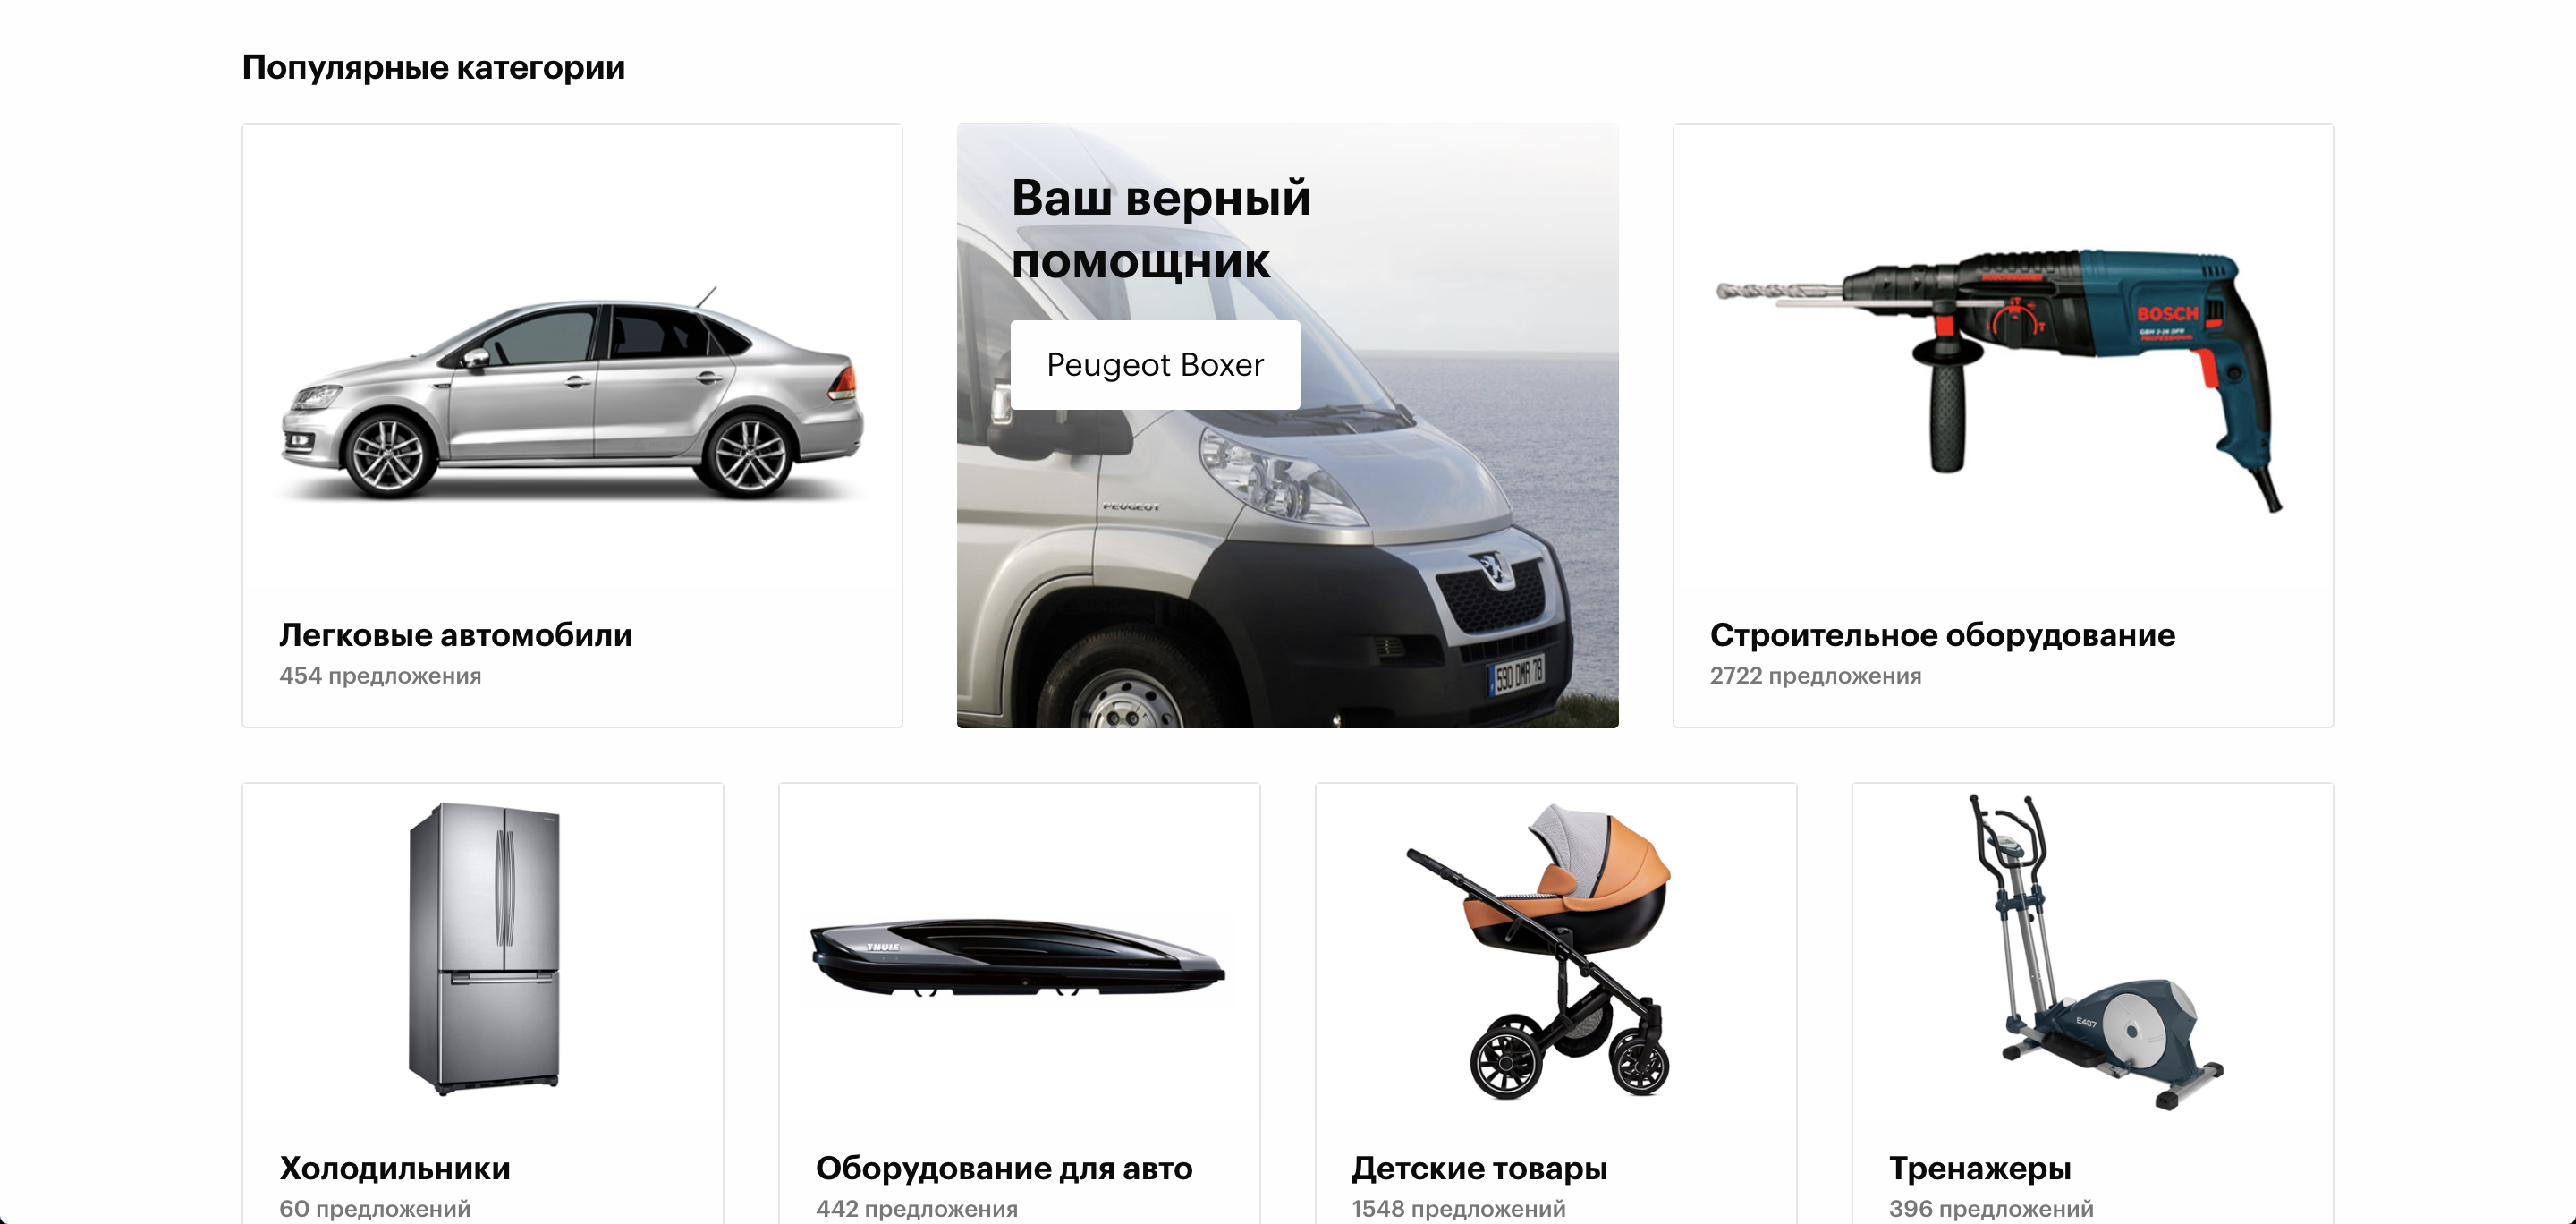
\includegraphics[scale=0.3]{analog_landing1.png}}
      \caption{Стартовая страница r24.by}
      \label{analogue:start}
\end{figure}

Данный сервис для аренды товаров рассчитан на покупку товаров у юридических лиц.
R24.by предоставляет разные тарифные планы для компаний, которые собираются продать товар:
\begin{enumerate}[label=\arabic*)]
  \item Базовый
  \begin{itemize}
    \item Неограниченное количество товаров;
    \item Размещение контактной информации;
    \item Доступ в личный кабинет;
    \item Цена: 0 руб/мес.
  \end{itemize}
  \item Стандарт
  \begin{itemize}
    \item Возможности “Базового” тарифа;
    \item Указание телефона на карточке товара;
    \item Бесплатное поднятие объявления раз в сутки;
    \item Цена: 22 руб/мес;
  \end{itemize}
  \item Премиум
  \begin{itemize}
    \item Возможности “Стандартного” тарифа;
    \item Одно прикрепленное объявление;
    \item Цена: 44 руб/мес
  \end{itemize}
\end{enumerate}
\bigbreak

Процесс регистрации представлен на рисунке \ref{analogue:reg}.
После заполнения всех полей в форме регистрации пользовтаель должен дождаться подтверждения от администрации сайта.
При успешном прохождении регистрации пользователю будет вышлен временный пароль для входа в учетную запись.

\begin{figure}[ht]
  \centering
      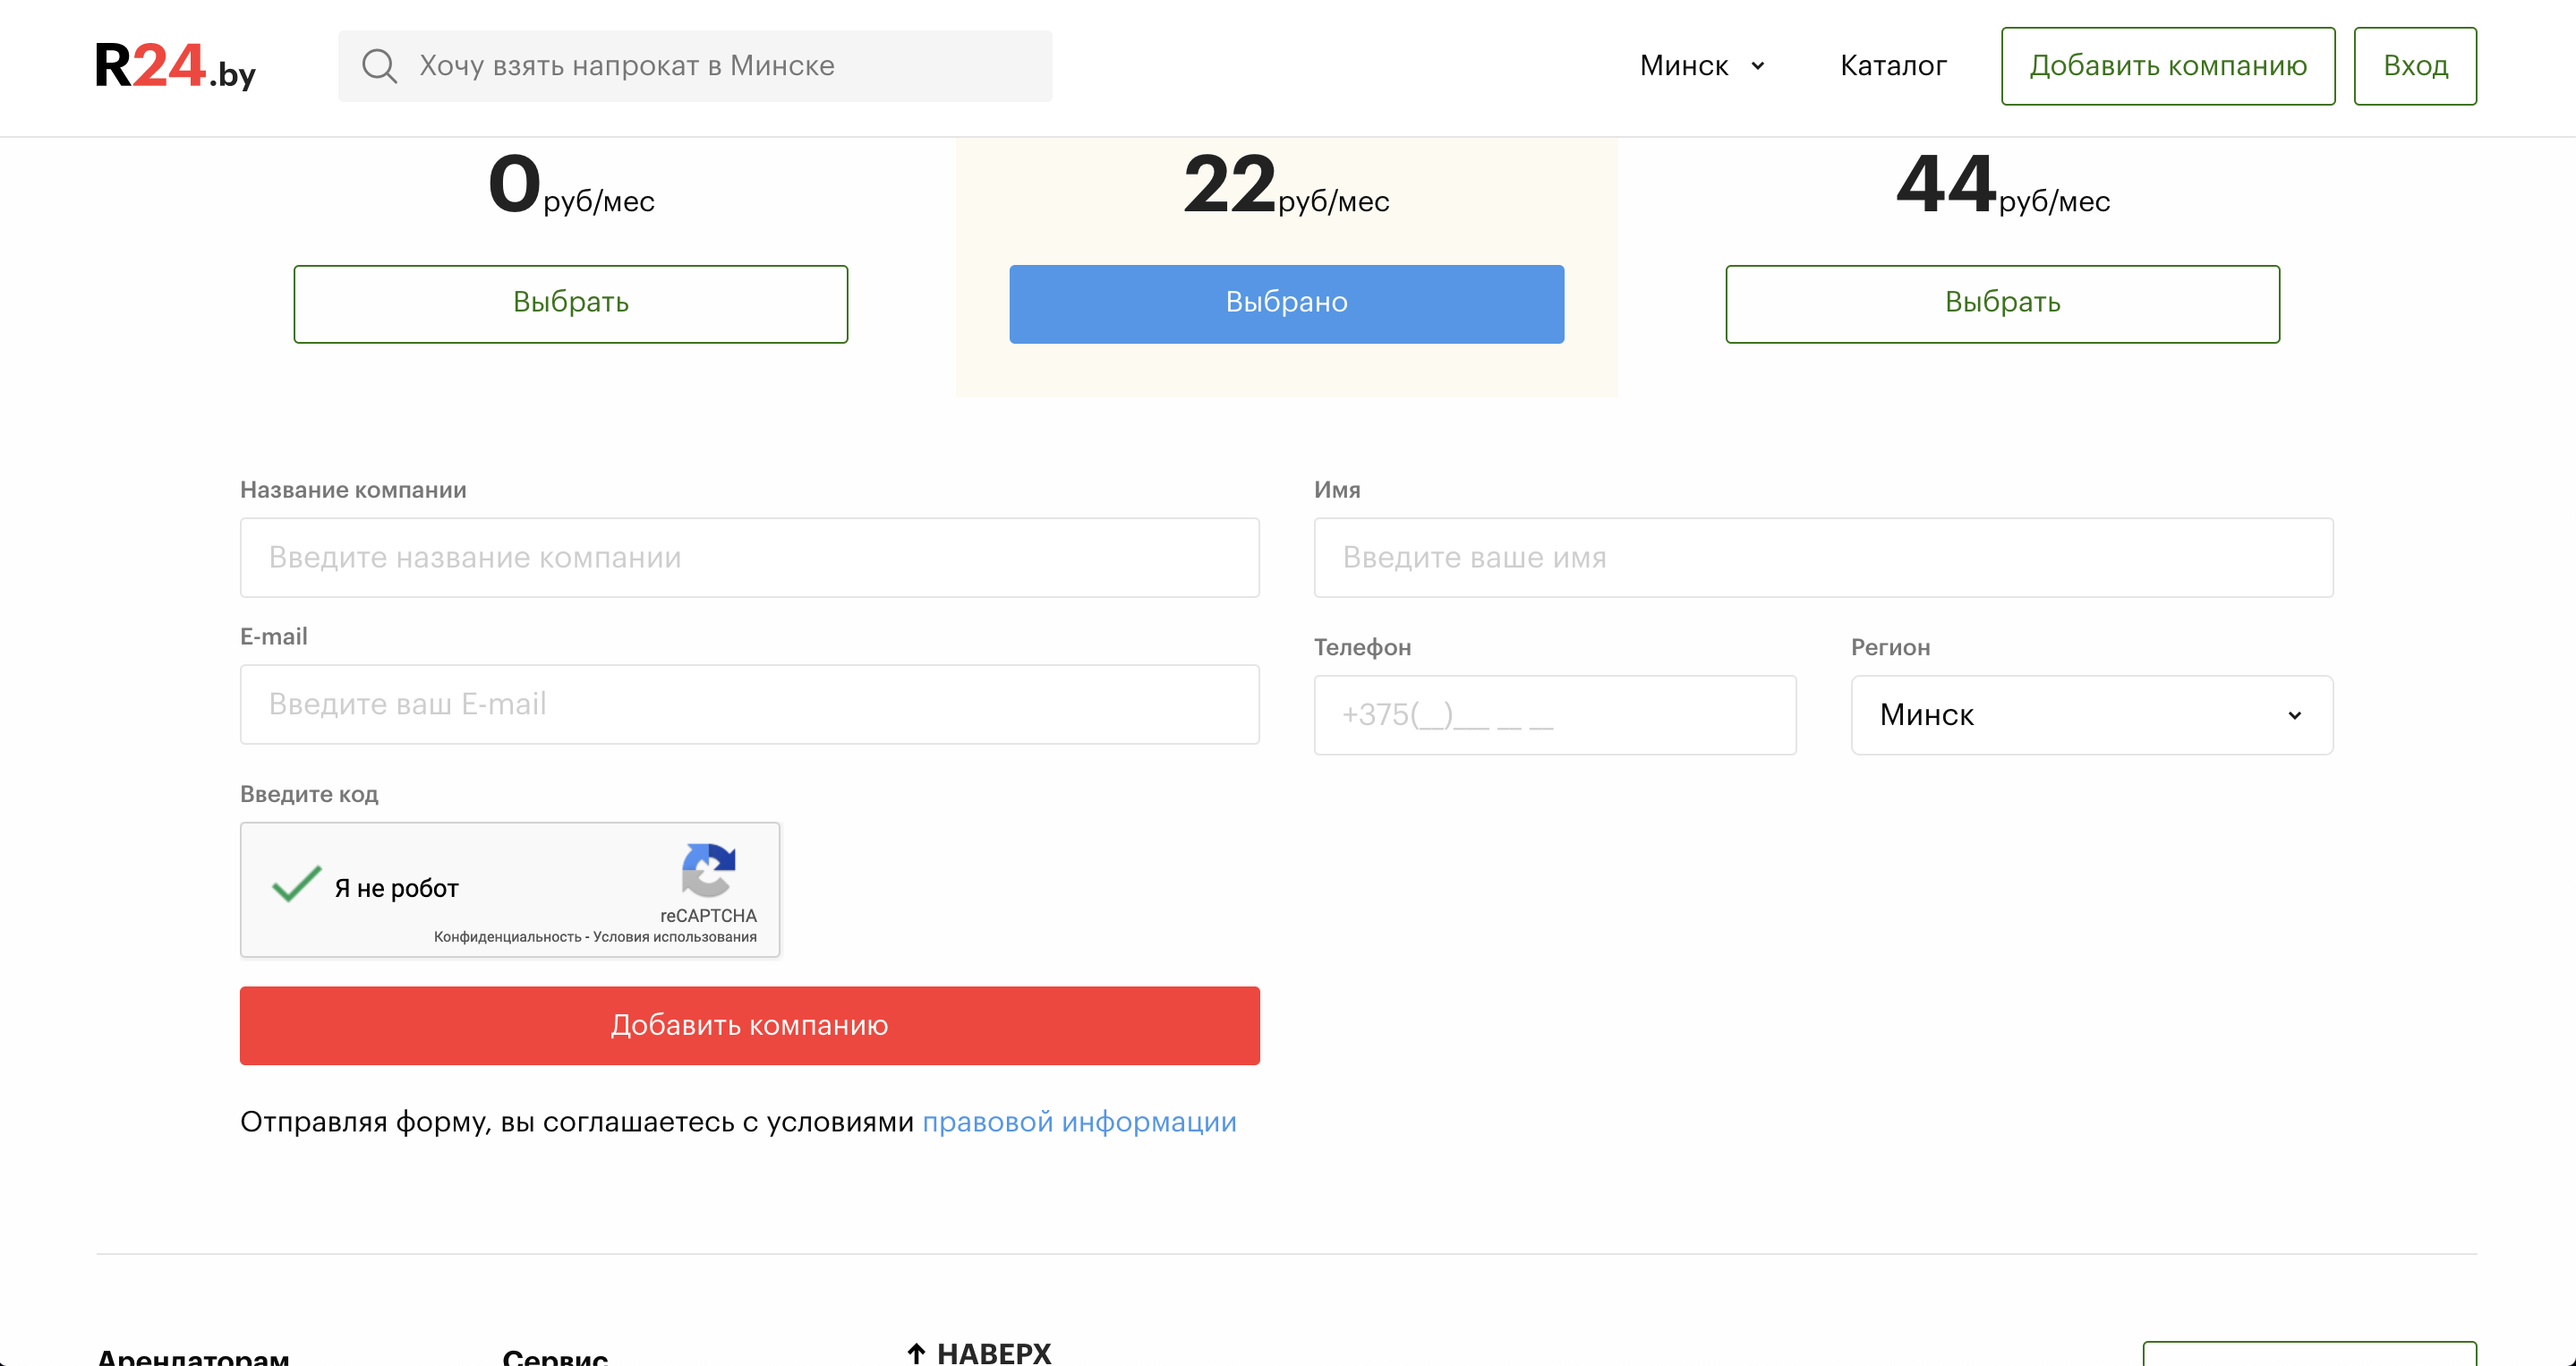
\includegraphics[scale=0.3]{analog_register.png}
      \caption{Страница регистрации r24.by}
      \label{analogue:reg}
\end{figure}

Как можно увидеть на рисунке \ref{analogue:search}, на стартовой странице сайта можно начать поиск товара по самым популярным категориям.
На данной странице сервис предоставляет возможность сортировать товары по убыванию либо возростанию цены.
Фильтрация заключается лишь в выборе срока сдачи товара в аренду.

\begin{figure}[ht]
  \centering
      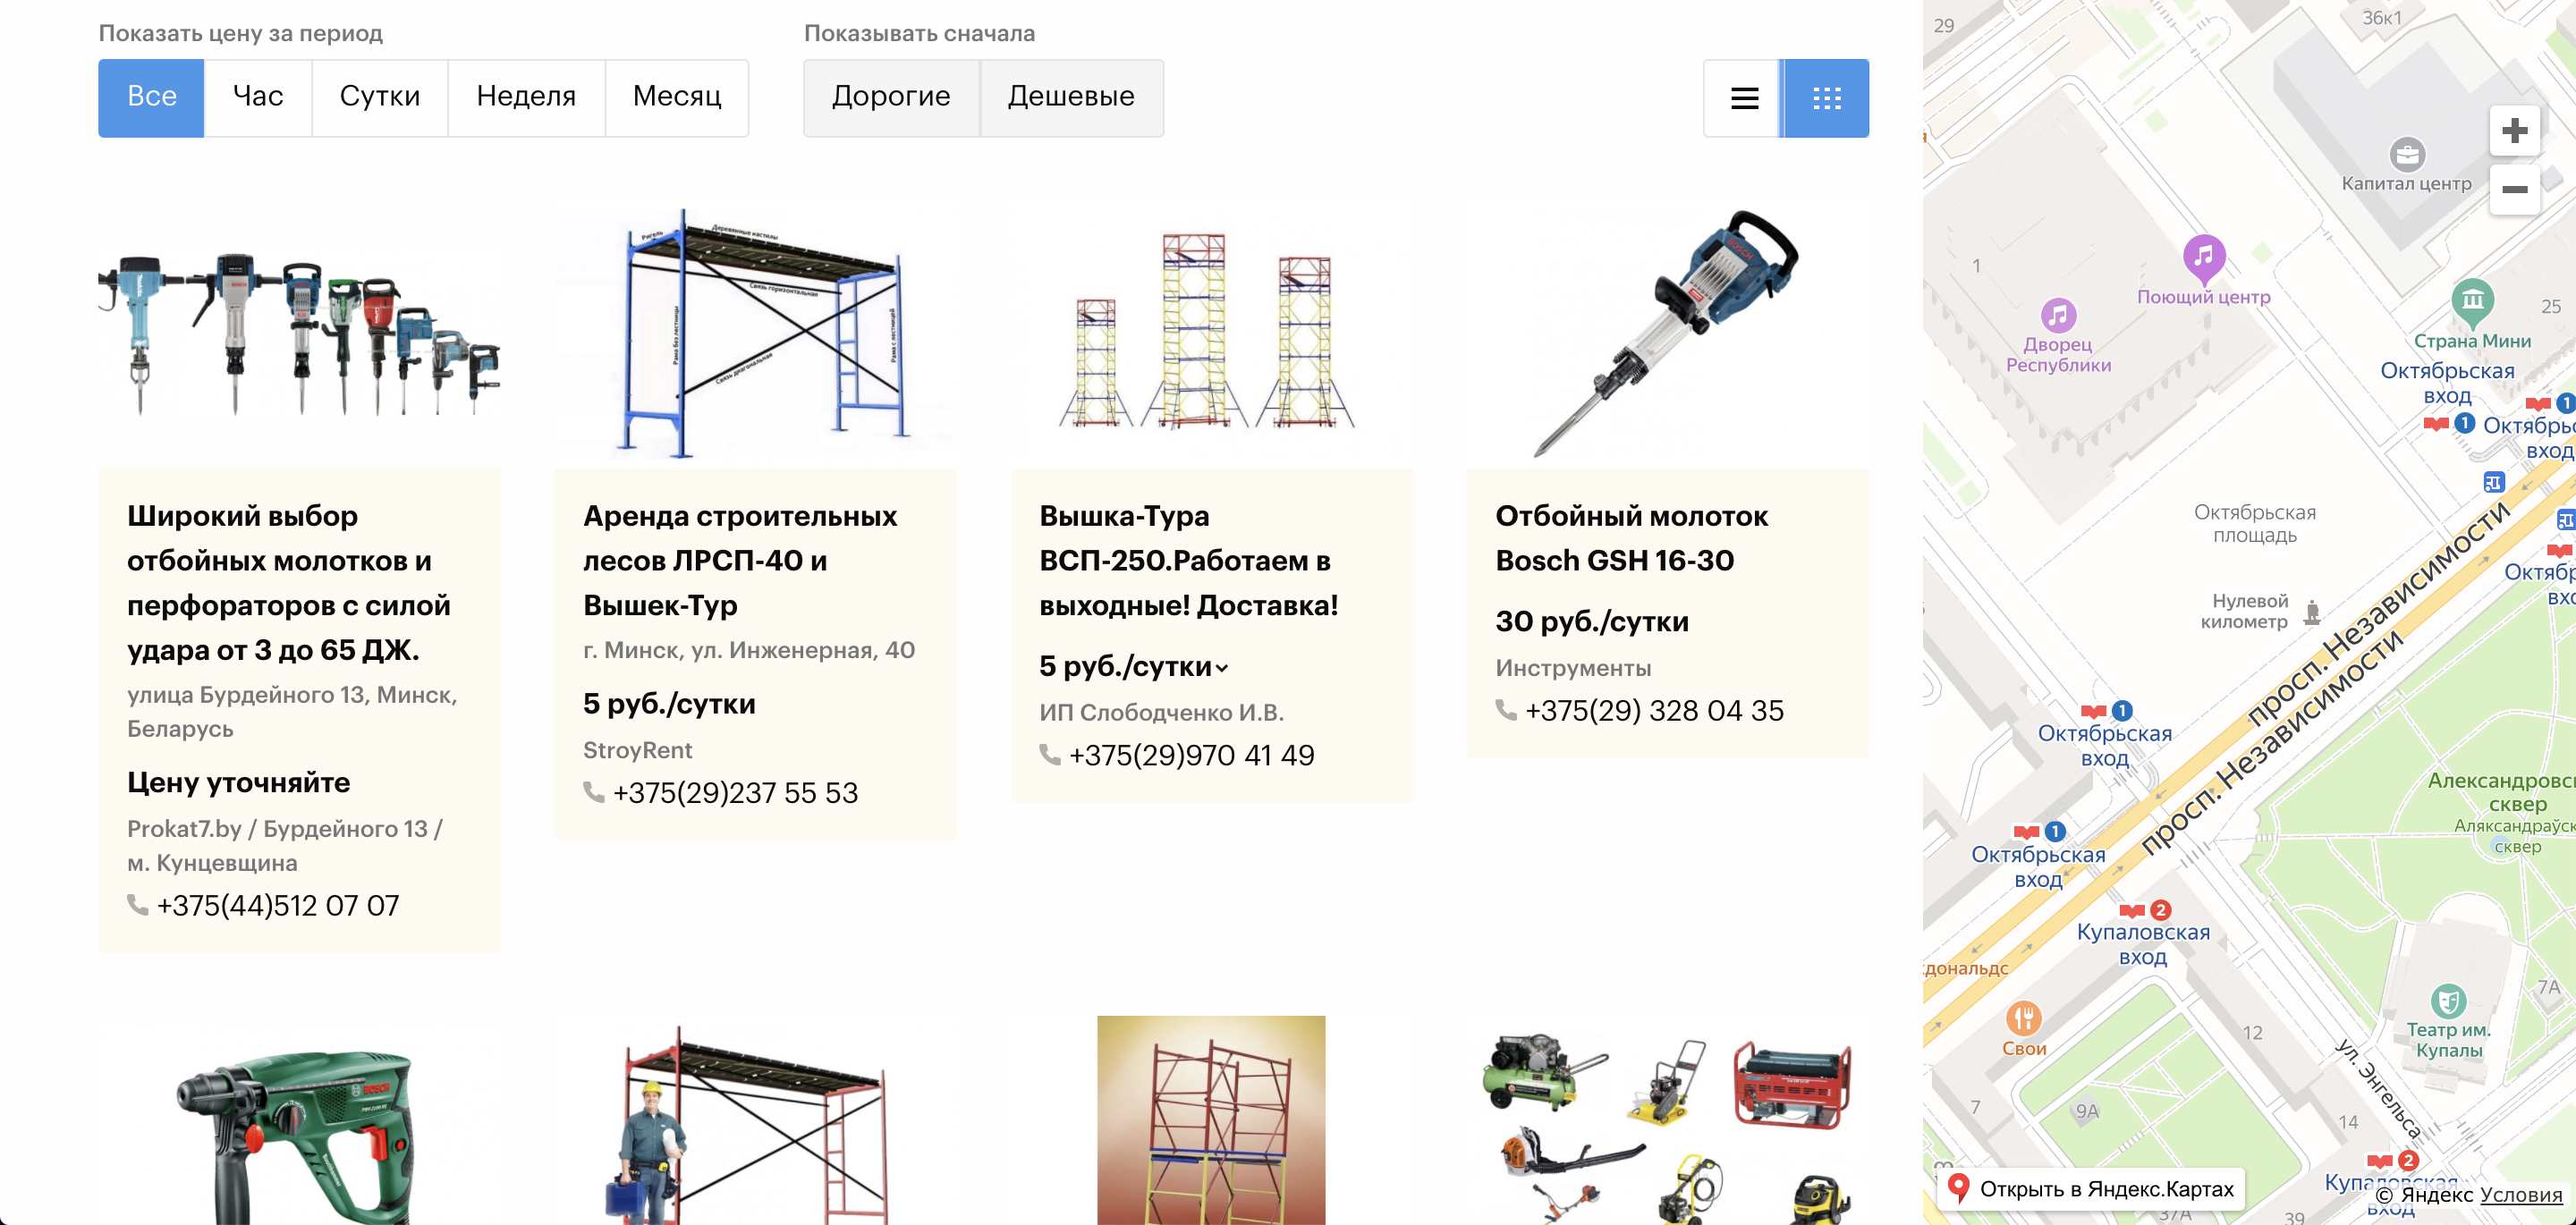
\includegraphics[scale=0.3]{analog_search.png}
      \caption{Страница поиска товаров r24.by}
      \label{analogue:search}
\end{figure}

На детально странице о товаре, представленной на рисутке \ref{analogue:det}, в отличие от странице поиска товаров представленно детальное описание товара.
Однако на сайте отсуствует корзина, либо личный кабинет.
Данный сайт представляет собой доску объявлений юридических лиц по предоставлению своих услуг.
Лишь на некоторых товарах присутствует кнопка для заказа обратного звонка.

\begin{figure}[ht]
  \centering
      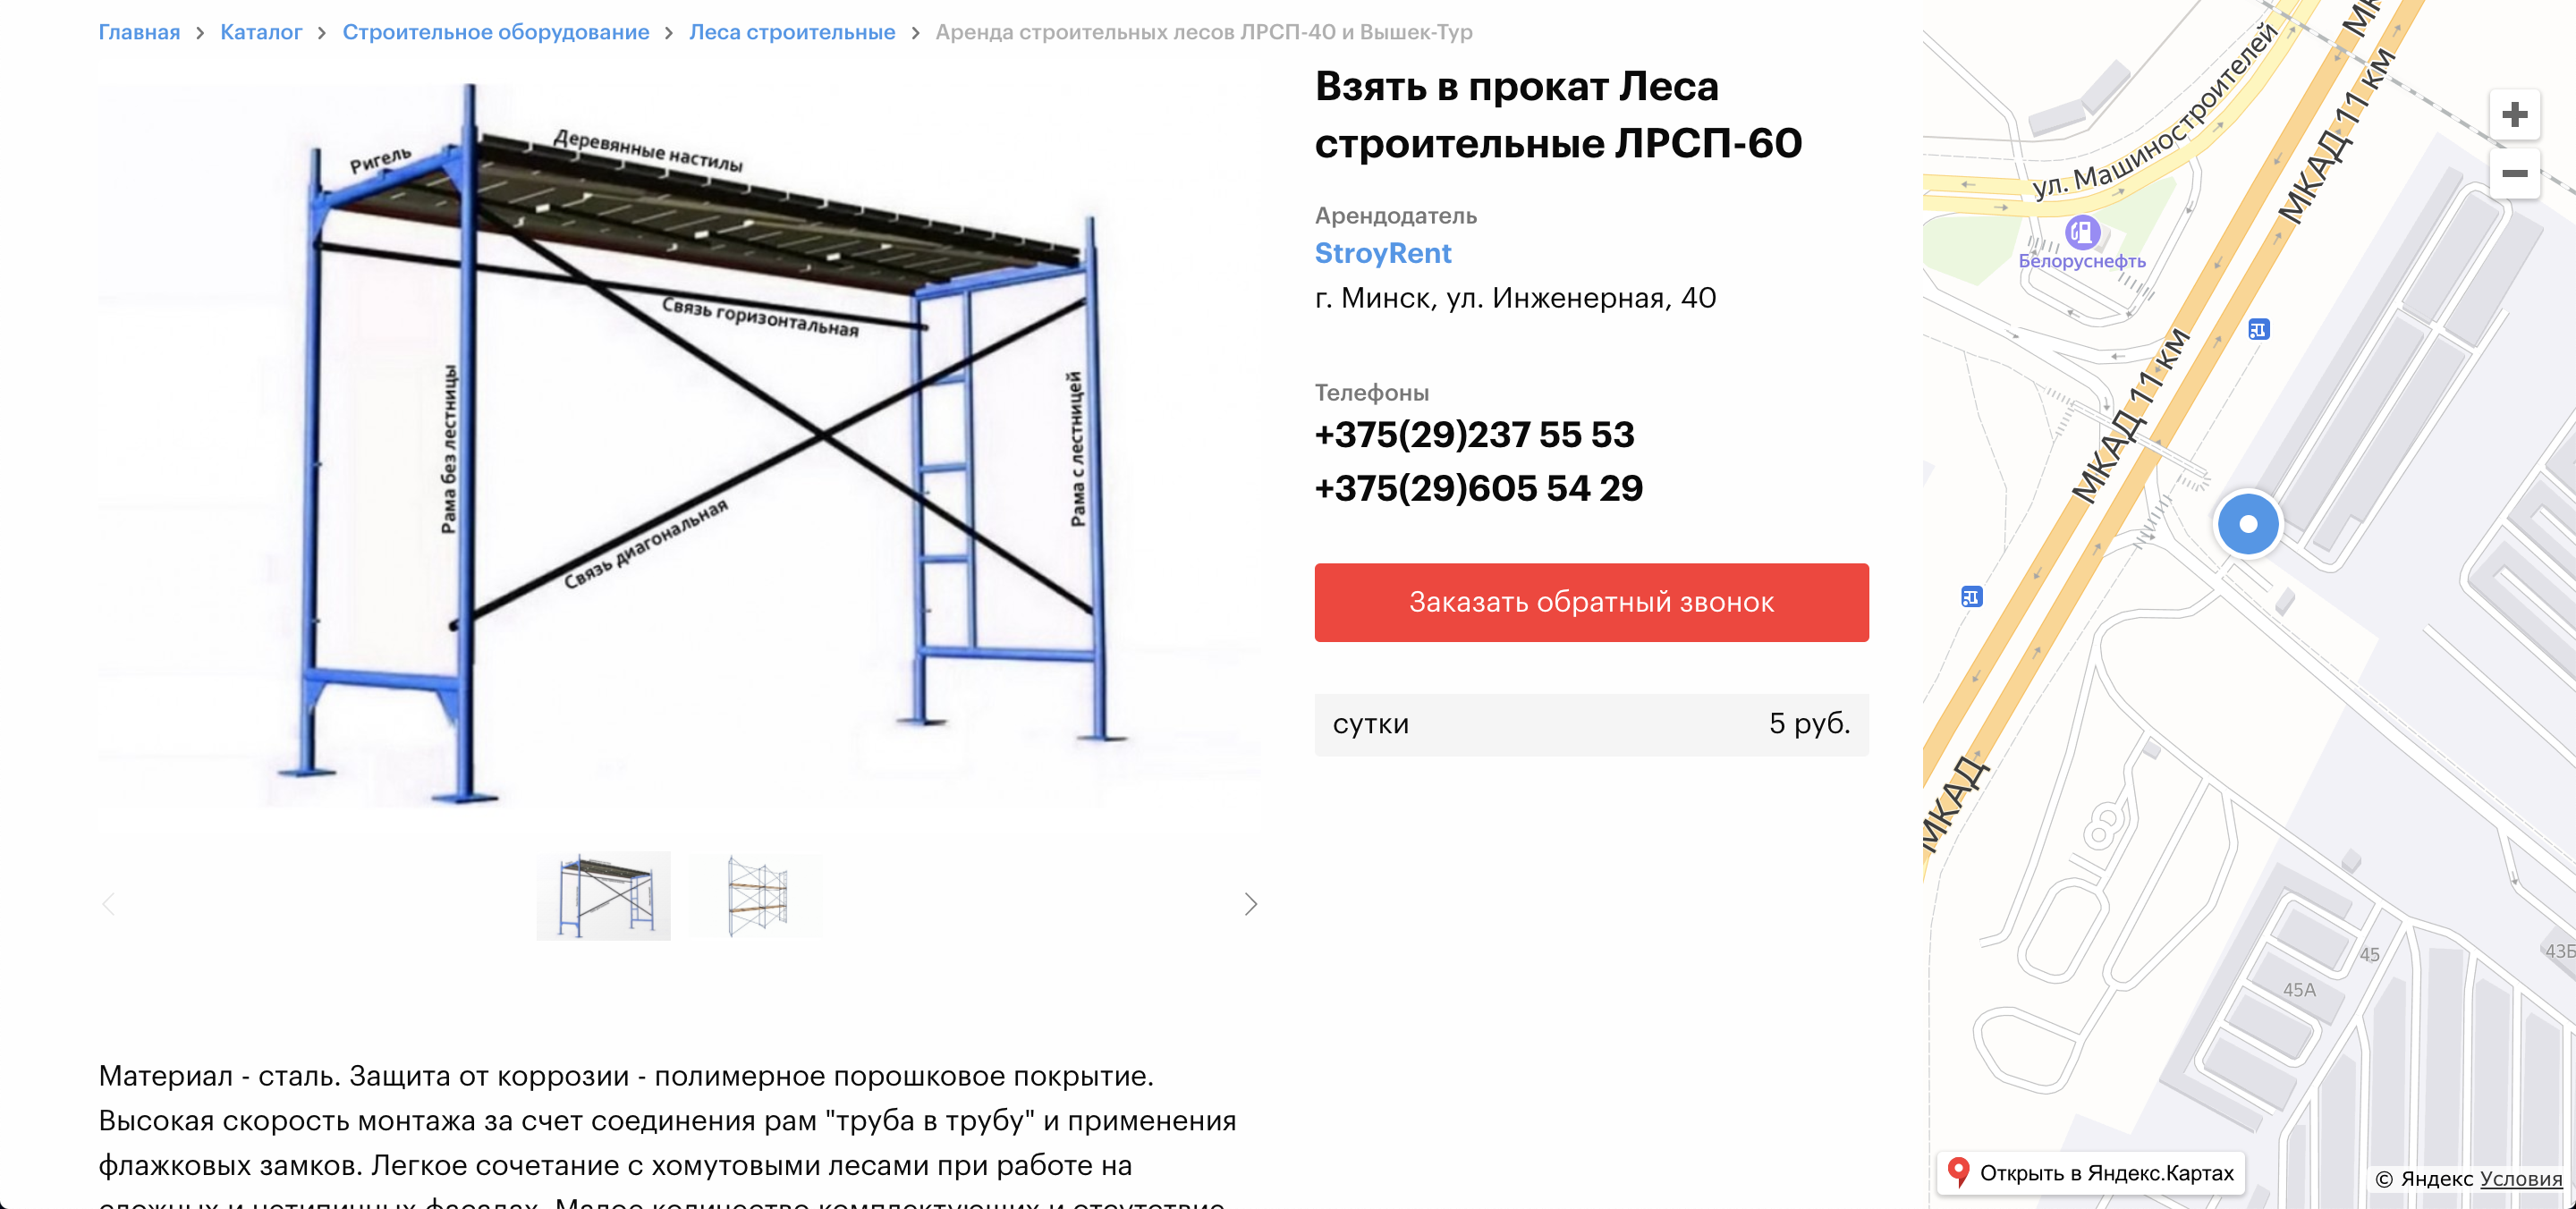
\includegraphics[scale=0.3]{analog_detail_item.png}
      \caption{Страница детализированного просмотра товара r24.by}
      \label{analogue:det}
\end{figure}

Таким образом можно прорезюмировать сайт r24.by:

Достоинства:
\begin{itemize}
  \item Данный сервис охватывает большой спектр товаров для разных потребностей;
  \item Наличие мобильной версии сайта;
  \item Возможность продвижения объявления.
\end{itemize}
\bigbreak
Недостатки:
\begin{itemize}
  \item Работает только в Гродно и Минске;
  \item Отсутствие отзывов о продавце;
  \item Отсутствие возможности организации продажи товаров физическими лицами;
  \item Отсутствие возможности покупки товара напрямую с сайта;
  \item Негибкая система сортировки и фильтрования товаров.
\end{itemize}


\subsection{Формулирование требований к програмному обеспечению}
По результатам изучения предметной области и обзора существующих систем-аналогов сформулируем требования к проектируемому программному средству.

\subsubsection{Основные функции}\hfill

Программное средство должно поддерживать следующие основные функции:
\begin{itemize}
  \item Регистрация и аутентификация;
  \item Возможность добавления товара на сайт;
  \item Возможность покупки товара на сайте;
  \item Возможность поиска товара;
  \item Управление пользовательской информацией;
  \item Управление товарами из интефейса администратора;
\end{itemize}

\subsubsection{Требования ко входным данным}\hfill

Входные данные для программного средства должны быть представлены в виде вводимого пользователем с помощью клавиатуры текста и выбора доступных опций пользовательского интерфейса.
Должны быть реализованы проверки вводимых данных на корректность с отображением информации об ошибках в случае их некорректности.

\subsubsection{Требования к выходным данным}\hfill

Выходные данные программного средства должны быть представлены посредством отображения информации с помощью различных элементов пользовательского интерфейса.

\subsubsection{Требования к временным характеристикам}\hfill

Производительность программно-аппаратного комплекса должна обеспечивать следующие временные характеристики: время реакции не запрос пользователя не должно превышать 2 секунд при минимальной скорости соединения 10 МБит/с.
Допускается невыполнение данного требования в слaчае, когда невозможность обеспечить заявленную производительность обу- словлена объективными внешними причинами.

\subsubsection{Требования к аутентификации пользователей}\hfill

Приложение должно мотивировать пользователя зарегистрировать в системе.
Данная мотивация будет возникать из-за невозможности неаутентифицированному пользователю осуществлять любые взаимодействия с товарами, в том числе их просмотр.

Регистрация пользователя должна происходить по номера телефона. Данный способ имеет ряд преимуществ:
\begin{enumerate}[label=\arabic*)]
    \item Идентификация пользователя;
    \item Возможность связаться с пользователем по мобильной связи;
    \item Отсутствие необходимости пользователю запоминать и вводить пароль от аккаунта.
\end{enumerate}

При утрате доступа к ранее зарегистрированному номеру телефона, у пользователя должна быть возможность связаться с администратором для изменения данных о номере телефона.

После прохождения процедуры подтверждения номера телефона пользователь должен указать данные о себе:
\begin{enumerate}[label=\arabic*)]
    \item ФИО;
    \item Место жительства, либо разрешить приложению использовать геолокацию и автоматически определить;
    \item Фотография;
    \item Адрес электронной почты(опционально).
\end{enumerate}

\subsubsection{Требования к организации процесса выставления товара на продажу в аренду}\hfill

При выставлении товара на продажу пользователь должен загрузить не менее одной фотографии продаваемого товара.
В описании товара должны быть указаны следующие характеристики:
\begin{enumerate}[label=\arabic*)]
    \item Год выпуска;
    \item Название;
    \item Состояние;
    \item Краткое описание товара;
    \item Возможность выкупа товара;
    \item Цена за один час аренды;
    \item Цена за одни сутки аренды;
    \item Возможность личной доставки арендодателем товара до арендатора;
    \item Категории товара.
\end{enumerate}

После размещения товара на платформе у пользователя есть возможность как скрыть товар из поисковой выдачи на неопределенное время, так и удалить товар из системы.
Приложение должно хранить все товары в реляционной базе Postgres с расширением Postgis, по причине возможности хранения координат.

\subsubsection{Требования к организации процесса поиски товаров в аренду}\hfill
Пользователь приложение должен иметь возможность в поиске товаров по их названию.

Пользователь должен иметь возможность фильтровать товары по категориям:
\begin{itemize}
    \item Состояние;
    \item Категории;
    \item Год выпуска;
    \item Возможность выкупа;
    \item Возможность личной доставки арендодателем товара до арендатора;
    \item Цена за час аренды;
    \item Цена за сутки аренды.
\end{itemize}

Пользователь должен иметь возможность сортировки товаров по одной из категорий:
\begin{itemize}
    \item Состояние;
    \item Цена за час аренды;
    \item Цена за сутки аренды;
    \item Год выпуска.
\end{itemize}

Поиск товаров должен быть реализован как выпадающий список фильтров и полей для сортировки.

При просмотре товаров списком пользователь видит только краткую информацию о товаре:
\begin{enumerate}[label=\arabic*)]
    \item Название;
    \item Цену за час;
    \item Цену за сутки;
    \item Первая фотография товара.
\end{enumerate}

Пользователь должен иметь возможность перейти на детальную страницу товара, где может увидеть все поля, которые заполнял продавец об этом товаре и ссылку на профиль самого продавца с возможностью перейти на профиль продавца.
На профиле продавца пользователь видит всю информацию, которую продавец заполнял о себе, а также список товаров, которые продавец продает.

Пользователь должен иметь возможность пожаловаться на продавца с описанием причины, если тот распространяет неудовлетворительные товары.

\subsubsection{Требования к организации процесса покупки товара}\hfill

При просмотре товара в процессе поиска пользователь должен иметь возможность добавить товар в корзину.
Так же при переходе на детальную информацию о товаре пользователь должен иметь возможность добавить товар в корзину.

Пользователь должен иметь возможность выбора способа доставки товара:
\begin{itemize}
    \item Лично забрать товар;
    \item Оформить доставку;
    \item Если была возможность доставки товара лично арендодателем, то выбрать ее.
\end{itemize}

Пользователь должен выбрать срок, на который он покупает товар в аренду.

При выборе доставки клиенту предоставляется итоговый счет за товар.
Пользователь должен иметь возможность согласиться с ценой и купить товар.
При успешной транзакции товар добавляется в к пользователю в раздел “у меня в аренде” с указанием, когда он должен его вернуть продавцу.
Продавцу приходит уведомление о том, что у него купили товар в аренду, после чего, соответствую выбранному способу доставки продавец должен доставить до покупателя товар.

При неудовлетворительном организации процесса продажи или покупки товара продавец или клиент должны иметь возможность пожаловаться администрации на пользователя приложения с описанием причины.

В промежутке от момента прохождения транзакции до возврата товара, пользователь должен иметь возможность оставить отзыв о продавце.
